\documentclass[a4paper]{bxjsarticle}  
\usepackage{zxjatype}
\usepackage[ipa]{zxjafont}

%% Use packages---------------------------------------------
\usepackage{hyperref}%\Hと喧嘩する
\usepackage{stmaryrd}%mapsfromとか

\usepackage{tcolorbox}%色付き枠
\usepackage{varwidth}%分かんないけどりちょますブログにあったやつ
\tcbuselibrary{breakable, skins, theorems}%あったやつ2

\usepackage{amsmath,amssymb}%数式全般
\usepackage{amsthm}%定理環境
\usepackage{mathrsfs}%花文字 (\mathscr)
\usepackage{bm}%ベクトルなどの太字 (\bm)
\usepackage{mathtools}%\coloneqq など
\usepackage{colonequals}%\colonequals
\usepackage{graphicx}%図の挿入
%\usepackage{subcaption}%関連する図を並べる
\usepackage{tikz}%図を描く
\usetikzlibrary{patterns}%網掛け等
\usepackage{tikz-cd}%可換図式を描く
\usepackage{cancel}%数式に斜線を引く
\usepackage{centernot}%\centernot
\usepackage{xparse}%凝ったマクロを作る (\NewDocumentCommand)
\usepackage{array,booktabs,float}%表組みなど
\usepackage{textcomp,gensymb}%\degree など
\usepackage{bbm}%\mathbbm で小文字や数字も太くなるようにする
\usepackage{listings}
\usepackage{url}
\usepackage[shortlabels]{enumitem}%番号付けを自動でさせる
\usepackage{color}%色を変える

%\divides, \notdivides を使えるようにする
\DeclareFontFamily{U}{matha}{\hyphenchar\font45}
\DeclareFontShape{U}{matha}{m}{n}{
<5> <6> <7> <8> <9> <10> gen * matha
<10.95> matha10 <12> <14.4> <17.28> <20.74> <24.88> matha12
}{}
\DeclareSymbolFont{matha}{U}{matha}{m}{n}
\DeclareMathSymbol{\divides}{3}{matha}{"17}
\DeclareMathSymbol{\notdivides}{3}{matha}{"1F}



\definecolor{frameinnercolor}{RGB}{49,44,44}

\newcounter{theorem}
\numberwithin{theorem}{subsection}% numberwithinはamsmath.styで定義されている
\newenvironment{theorem}[2][]{%
%#1 = タイトル, #2 = 定理環境名
\refstepcounter{theorem}%

\newtcolorbox{theobox}[1][]{%
enhanced,
coltitle=black,colback = white,colframe = green!35!black,fonttitle=\bfseries,
sharp corners=all,
breakable=true,
top=4mm,
before skip=2mm,
attach boxed title to top left={yshift=-3mm,xshift=5mm},
boxed title style={colback=white,boxrule=1pt},
title=##1,
}

\ifstrempty{#1}{% ifstremptyはetoolbox.styで定義.etoolbox.styはtcolorboxが読み込むので宣言不要
\begin{theobox}[#2~\thetheorem.]}
{\begin{theobox}[#2~\thetheorem:~{#1}]}
}{\end{theobox}}


\newenvironment{thm}[1][]
{\begin{theorem}[#1]{定理}
}{\end{theorem}}
\newenvironment{prop}[1][]
{\begin{theorem}[#1]{命題}
}{\end{theorem}}
\newenvironment{defi}[1][]
{\begin{theorem}[#1]{定義}
}{\end{theorem}}
\newenvironment{rem}[1][]
{\begin{theorem}[#1]{注意}
}{\end{theorem}}
\newenvironment{eg}[1][]
{\begin{theorem}[#1]{例}
}{\end{theorem}}
\newenvironment{lem}[1][]
{\begin{theorem}[#1]{補題}
}{\end{theorem}}
\newenvironment{cor}[1][]
{\begin{theorem}[#1]{系}
}{\end{theorem}}
\newenvironment{rev}[1][]
{\begin{theorem}[#1]{復習}
}{\end{theorem}}
\newenvironment{conj}[1][]
{\begin{theorem}[#1]{予想}
}{\end{theorem}}
\newenvironment{fact}[1][]
{\begin{theorem}[#1]{事実}
}{\end{theorem}}

\numberwithin{equation}{section}

%黒板文字
\newcommand{\N}{\mathbb{N}}%自然数
\newcommand{\Z}{\mathbb{Z}}%整数
\newcommand{\Q}{\mathbb{Q}}%有理数
\newcommand{\R}{\mathbb{R}}%実数
\newcommand{\C}{\mathbb{C}}%複素数
\newcommand{\T}{\mathbb{T}}%トーラス

%カリグラフィー
\newcommand{\F}{\mathcal{F}}%フィルターか完全加法族
\newcommand{\g}{\mathfrak{g}}
\newcommand{\h}{\mathfrak{h}}
\renewcommand{\a}{\mathfrak{a}}
\newcommand{\X}{\mathfrak{X}}%ベクトル場
\newcommand{\A}{\mathcal{A}}
\renewcommand{\O}{\mathcal{O}}

%引数持ち
\newcommand{\abs}[1]{\left\lvert#1\right\rvert}%絶対値
\newcommand{\norm}[1]{\left\lVert#1\right\rVert}%ノルム
\newcommand{\diff}[2]{\frac{d#1}{d#2}}%微分
\newcommand{\pdiff}[2]{\frac{\partial #1}{\partial #2}}%偏微分
\newcommand{\set}[2]{\{\, #1\mid #2\,\}}%集合
\newcommand{\nikou}[2]{\prescript{#1}{}{\mathrm{C}}_{#2}}%二項係数
\newcommand{\inpro}[1]{\left\langle #1 \right\rangle}%内積
\newcommand{\tensor}[2]{#1\otimes\overline{#2}}

%引数無し
\newcommand{\im}{\mathrm{Im}}
\renewcommand{\ker}{\mathrm{Ker}}
\renewcommand{\hom}{\mathrm{Hom}}
\newcommand{\act}{\curvearrowright}
\newcommand{\siji}{\mathbbm{1}}
\newcommand{\clspan}{\overline{\mathrm{Span}}}
\newcommand{\spn}{\mathrm{Span}}
\newcommand{\mapin}{\rotatebox{90}{$\in$}}
\newcommand{\id}{\mathrm{id}}
\newcommand{\tr}{\mathrm{Tr}}

%全単射示すやつ
\newcommand{\mapstodown}{\raise.63286ex\hbox{$\mathcal{7}-$}\mspace{-16mu}\lower.62916ex\hbox{$\leftarrow$}\mspace{-13mu}\supset}
\newcommand{\mapsfromdown}{\reflectbox{\mapstodown}}
\newcommand{\mapstoup}{\rotatebox[origin=c]{180}{$\mapsfromdown$}}
\newcommand{\mapsfromup}{\rotatebox[origin=c]{180}{$\mapstodown$}}
%%------------------------------------------------------
\title{Lie群論のノート}
\author{@buta\_kimchi\_\thanks{\url{https://twitter.com/buta_kimchi_}}}
\date{\today}
\begin{document}
\maketitle
\begin{abstract}
    Warnerの ``Foundations of Differentiable Manifolds and Lie Groups'' と Fulton-Harrisの私的ノート。
\end{abstract}
\tableofcontents

\newpage
\section{多様体}
多様体には第二可算性を課す。

\subsection{はめ込まれた部分多様体}
記法がややクソかもしれない。
\begin{rem}[記法]
    多様体は$M,N$、(はめ込まれた)部分多様体は$\iota:P\hookrightarrow M$、$C^\infty$級写像は$\phi,\psi:M\to N$、$C^\infty$級関数は$f,g:M\to\R$。近傍はどの点の周りかを表して$U_p,U_q$などと書く。局所座標は$\tau,\sigma:U\to\R^n$などを使い、簡単のため像は常に$\R^d$全体とする。
\end{rem}
逆関数定理はあればあるほど良い。
\begin{rem}[逆関数定理]
    多様体$M,N$とその間の$C^\infty$級写像$\phi:M\to N$と$p\in M,\ q:=\phi(p)$について
    \begin{enumerate}[(1)]
        \item 微分$d\phi_p:T_pM\to T_qN$が単射なら、ある局所座標$(U_p,\tau),(U_q,\sigma)$が存在し
        \[\R^d\xrightarrow[\tau^{-1}]{\cong} U_p\xrightarrow{\phi}U_q\xrightarrow[\sigma]{\cong}\R^c\ =\ \R^d\hookrightarrow\R^c\]
        とできる。ここで、$\R^d\hookrightarrow\R^c$とは標準的な包含写像である。
        \item 微分$d\phi_p:T_pM\to T_qN$が全射なら、ある局所座標$(U_p,\tau),(U_q,\sigma)$が存在し
        \[\R^d\xrightarrow[\tau^{-1}]{\cong} U_p\xrightarrow{\phi}U_q\xrightarrow[\sigma]{\cong}\R^c\ =\ \R^d\twoheadrightarrow\R^c\]
        とできる。ここで、$\R^d\twoheadrightarrow\R^c$とは標準的な全射である。
    \end{enumerate}
    つまり、局所的には自明な線形写像にできる、ということである。
\end{rem}


\begin{rem}[部分多様体]
    はめ込まれた部分多様体を単に「部分多様体」と呼ぶ。つまり、$\iota:P\hookrightarrow M$について
    \begin{center}
        はめ込み$\Leftarrow$単射なはめ込み$\Leftarrow$埋め込み
    \end{center}
    という論理包含があるが、この真ん中を満たす$\iota$を部分多様体と呼ぶ。恐らく、埋め込みを部分多様体と呼ぶのが平均的な定義だと思うが、わざわざそれよりも弱い定義を採用するのは理由がある。後述するFrobeniusの定理によって自然に表れる極大積分多様体という対象は埋め込みにならないからである。
\end{rem}
はめ込みは各点の微分が単射であることで、埋め込みは像への同相を誘導するはめ込みであった。しかし、これだけだとあまり思い出せた気がしないので簡単な例を軽く紹介する。
\begin{eg}[not はめ込み]
    $\iota:\R\ni x\longmapsto x^3\in\R$ という写像ははめ込みでない。しかし同相ではある。
\end{eg}
\begin{eg}[はめ込み but not 部分多様体]
    自己交叉するものは全てこれである。矢印は曲線の向きを表す。
    \[\begin{tikzpicture}
        \draw (1,1) to [out=-135,in=-90] (-2,0);
        \draw[->] (-2,0) to [out=90,in=135] (1,-1);
    \end{tikzpicture}\]
\end{eg}
\begin{eg}[部分多様体 but not 埋め込み]
これが一番重要である。前者は悪いが後者は良い部分多様体である。
    \begin{itemize}
        \item 8の字のやつ(どちらも$\R$からの像であって$\to\pm\infty$で原点に近づくが、近づく方向が違う)
        \[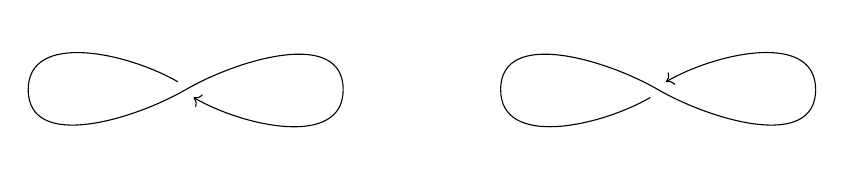
\begin{tikzpicture}
            \draw (-3-0.1,0.1) to [out=150,in=90] (-3-2,0);
            \draw (-3-2,0) to [out=-90,in=-150] (-3,0);
            \draw (-3,0) to [out=30,in=90] (-3+2,0);
            \draw[->] (-3+2,0) to [out=-90,in=-30] (-3+0.1,-0.1);
            
            \draw (3-0.1,-0.1) to [out=-150,in=-90] (3-2,0);
            \draw (3-2,0) to [out=90,in=150] (3,0);
            \draw (3,0) to [out=-30,in=-90] (3+2,0);
            \draw[->] (3+2,0) to [out=90,in=30] (3+0.1,0.1);
        \end{tikzpicture}\]
        \item トーラスにめっちゃ巻き付くやつ。$\iota:\R\ni t\longmapsto(\exp(2ti),\exp(2\alpha ti))\in \T^2$ を$\alpha\in\R\setminus\Q$について考えると、稠密になって滅茶苦茶な絵になる。
        \[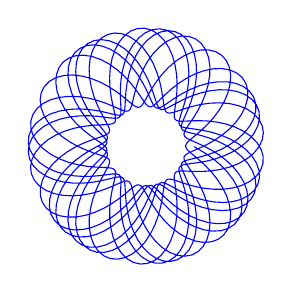
\begin{tikzpicture}
            \draw[blue,samples=1000,domain=-9*pi:10*pi,variable=\theta] plot(\theta r:{0.5+sin(1.79*\theta r)^2});
            
        \end{tikzpicture}\]
    \end{itemize}
    後者の良い部分多様体に主に興味がある。これは$X:=\pdiff{}{\theta_1}+\alpha\pdiff{}{\theta_2}$というベクトル場の積分曲線であるが、Frobeniusの定理は積分曲線の次元を上げた(つまり$c$個のベクトル場を積分してできる$c$次元の部分多様体)についての定理である。
\end{eg}
部分多様体$\iota:P\hookrightarrow M$は単射だから、$\iota$とは$M$の部分集合$P$上での多様体構造のことと言ってもよい。「$P\subset M$がはめ込まれた部分多様体」という言明は$P$上の位相とか微分構造を指定しないと意味をなさない一方、「$P\subset M$が埋め込まれた部分多様体」という言明は意味をなす。
\begin{rem}[埋め込みの特徴付け]
    $P\subset M$が埋め込み$\iff$局所的に$(P,M)$は$(\R^c,\R^d)$に微分同相。\\
    つまり、$\forall p\in P\ \exists(U_p,\tau)\ \tau(U_p\cap P)=\R^c\times\{0\}$ となること。
\end{rem}
\begin{eg}[複数の位相が入る部分多様体]
    $M:=\R^2,\ P$を8の字とする。図のように二通り$\R$からの$C^\infty$像だと思える
    \[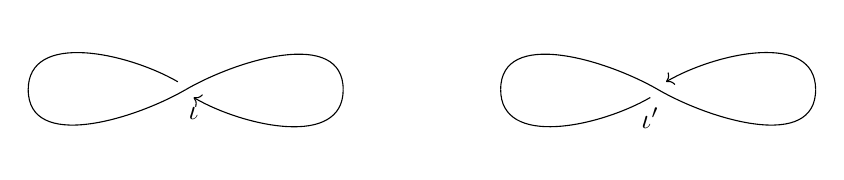
\begin{tikzpicture}
        \draw (-3-0.1,0.1) to [out=150,in=90] (-3-2,0);
        \draw (-3-2,0) to [out=-90,in=-150] (-3,0);
        \draw (-3,0) to [out=30,in=90] (-3+2,0);
        \draw[->] (-3+2,0) to [out=-90,in=-30] (-3+0.1,-0.1)node[below]{$\iota$};
        
        \draw (3-0.1,-0.1)node[below]{$\iota'$} to [out=-150,in=-90] (3-2,0);
        \draw (3-2,0) to [out=90,in=150] (3,0);
        \draw (3,0) to [out=-30,in=-90] (3+2,0);
        \draw[->] (3+2,0) to [out=90,in=30] (3+0.1,0.1);
    \end{tikzpicture}\]
    が、$\iota'=\iota\circ\text{hoge}$となる$\R$の微分同相hogeは存在しない。
    \[\begin{tikzcd}
        \R\arrow[dr,"\not\exists\ \text{hoge}"'] \arrow[r,"\iota'"] & \R^2\\
	&	\R\arrow[u,"\iota"]
    \end{tikzcd}\]
\end{eg}
しかし、実は次が成立する。
\begin{prop}\label{prop:111}
	\begin{enumerate}[(a)]
		\item $P(\subset M)$上の位相を一つ固定する。この位相と整合する$C^\infty$構造であって、$P\hookrightarrow M$が部分多様体となるようなものは高々一意である。
		\item $P(\subset M)$が埋め込みであるとする。このとき$P$を部分多様体とする$P$上の多様体としての構造(位相も取り換えて良い)は、$M$の微分構造から誘導されるもの($P$を埋め込みとするもの)だけである。
	\end{enumerate}
	つまり、部分多様体$P\subset M$とは本来「$P$と$P$の位相、$P$の微分構造」を指定しなければいけないところを、「$P$と$P$の位相」だけを指定すれば十分ということである。更に、埋め込まれた部分多様体は埋め込まれていない部分多様体になりえないのである。
\end{prop}
これを示す前に、準備として次の定理を証明する。
\begin{thm}
	部分多様体$\iota:P\hookrightarrow M$と$C^\infty$級写像$\phi:N\to M$に対し$\phi(N)\subset\iota(P)$となっていたとする。
	\[\begin{tikzcd}
	    N\arrow[r,"\phi"]\arrow[dr,"\phi_0"'] &M\\
	    & P\arrow[u,hook,"\iota"']
	\end{tikzcd}\]
	\begin{enumerate}[(a)]
	    \item $\phi_0$が連続$\Rightarrow \phi_0$が$C^\infty$級
	    \item $\iota:P\hookrightarrow M$が埋め込み$\Rightarrow \phi_0$は連続
	\end{enumerate}
\end{thm}
特に、埋め込みの場合は自動的に$\phi_0$は滑らかである。
\begin{proof}
    (b)は相対位相の普遍性である。(a)を示す。\\
    $n\in N$を取り、$p:=\phi_0(n),\ m:=\iota(p)$とし、近傍$U_n,U_p,U_m$を十分小さく取って$U_m\subset \iota(U_p),\ U_p\subset \phi_0(U_n)$とできる。$d\iota_p$は単射だから、逆関数定理より次を満たす$r:U_m\to P$が取れる。
    \[U_p\overset{\iota}{\longrightarrow}U_m\overset{r}{\longrightarrow}P\ =\ U_p\hookrightarrow P\]
    つまり、標準的な包含$\R^d\hookrightarrow\R^c$が左逆写像を持つことから、それの両側に微分同相を掛けた$\iota\lvert_U$も左逆写像を持つことになる、ということである。このような$r$の作り方から$r$は$C^\infty$級であり、$\phi_0$も$C^\infty$級。
    \[\phi_0\lvert_{U_n}=r\circ\iota\circ \phi_0\lvert_{U_n}=r\circ \phi\lvert_{U_n}\]
\end{proof}
\begin{proof}[Proof of 命題\ref{prop:111}]
    (a)は上の定理の(a)からすぐに従う。与えられた$P$上の位相と整合的な極大アトラス$\A_1,\A_2$に対し、$N,P$を$(P,\A_1),(P,\A_2)$とすれば $\id_P$が$C^\infty$となる。
    \[\begin{tikzcd}
        (P,\A_1)\arrow[r,hook]\arrow[dr,"\id"'] &M\\
	    & (P,\A_2)\arrow[u,hook]
    \end{tikzcd}\]
    $\A_1,\A_2$を入れ替えたら$\id_P$が微分同相になり、つまり$\A_1=\A_2$となる。\\
    (b)を示す。$P$上の多様体構造$(P,\O,\A)$であって包含写像$P\hookrightarrow M$が部分多様体になるものを取る。上の定理の(b)から$\id:(P,\O,\A)\to P$は$C^\infty$級になる。可読性のため、$\id=:\phi$と置く。
    \[\begin{tikzcd}
        (P,\O,\A)\arrow[r,hook]\arrow[dr,"\phi"'] &M\\
	    & P\arrow[u,hook]
    \end{tikzcd}\]
    この図式を微分に落とすと、部分多様体からの包含写像の微分は単射であり、可換性から$d\phi$は単射。
    \[\begin{tikzcd}
        (P,\O,\A)_p\arrow[r,hook]\arrow[dr,"d\phi"'] &M_p\\
	    & P_p\arrow[u]
    \end{tikzcd}\]
    今$f:(P,\O,\A)\to P$は全単射で微分が各点で単射。より一般にこういう状況においては、第二可算性から$\phi$の微分同相性が出てくる\footnote{第二可算性を課さない場合、連続体濃度の集合に離散位相を入れた0次元多様体は$\R$への全単射なはめ込みを持つ。}。なぜなら、$\phi:M\to N$について$M$の方が真に$N$より次元が低ければ像は$N$内で測度零になる。一方、次元が等しければ、微分$d\phi$は同じ次元の間の線形単射であり線形同型となる。
\end{proof}
\begin{defi}[スライス]
    $(U,\tau)$を$M$の局所座標とする。$\tau=(x_1,\dots,x_d)$と成分表示する($x_i:M\to\R$)。\\
    各$a\in\R^{d-c}$について
    \[S_a:=\tau^{-1}(\R^c\times\{a\})=\{(x_{c+1},\dots,x_d)=a\}\]
    という形の$U$の部分集合をスライスと呼ぶ。
\end{defi}
\begin{prop}[はめ込みは局所的にスライス]\label{prop:112}
    はめ込み$\iota:P\to M$について、各$p\in P$の近傍$U_p$で$\iota:U_p\to\iota(U_p)$が微分同相になるものが取れる。つまり、部分多様体は幾つかのスライスの和集合で書け、それらをアトラスとするようにできる。
\end{prop}
しかし、8の字の部分多様体を思い出すと分かる通り、$\iota(P)$に含まれるスライスが全て$P$の開集合になるとは限らない。
\begin{proof}
    逆関数定理から即座に従う。
\end{proof}
\begin{thm}[正則値定理]
    $\phi:M\to N$と部分多様体$\iota:Q\hookrightarrow N$に対し、$P:=\phi^{-1}(\iota(Q))$と置く。
    \[\begin{tikzcd}
        M\arrow[r,"\phi"] &N\\
        P\arrow[u,hook]\arrow[r,"\phi"] &Q\arrow[u,hook,"\iota"']
    \end{tikzcd}\]
    $\forall p\in P\ N_{\phi(p)}=d\phi(M_p)+d\iota(Q_{\phi(p)})$ のとき、$P$には自然に多様体構造が入り、$P\hookrightarrow M$は部分多様体、$\phi:P\to Q$は$C^\infty$級になる。更に、$Q\subset N$が埋め込みのとき$P\subset M$も埋め込みになる。
\end{thm}
これの$Q$が一点の場合がよく知られた正則値定理(このpdfだと単に逆関数定理と呼んでいるが)である。
\begin{proof}
    $P:=\set{(m,q)\in M\times Q}{\phi(m)=\iota(q)}$ と置く。つまり、これと$\phi^{-1}(\iota(Q))$に自然な全単射($M$成分だけから復元できる)があるが、$P$の多様体としての構造を$M\times Q$から誘導させる。という操作が許されるのは$P\subset M\times Q$が埋め込みになっている場合くらいだが、ちゃんとそれが成り立つことが確認できる。\\
    局所的に$P\subset M\times Q$が線形空間の自明な包含に微分同相であることを示せばいいから、$M,Q,N$は全てユークリッド空間$M=\R^a,Q=\R^b,N=\R^c$として良い。このとき$P$は次の写像の$\{0\}$の逆像。
    \[F:M\times Q=\R^a\times\R^b\ni(m,q)\longmapsto \phi(m)-\iota(q)\in\R^c=N\]
    各$P$の点でのこれの微分が全射になることが仮定だったから、逆関数定理より$F$は全射線形写像にとしてよい。つまり、座標を取れば$P=\ker F\subset M\times Q$という線形空間の包含にできるからOK。\\
    $P$から$M,Q$への写像は成分への射影で得られる。$P\hookrightarrow M$が部分多様体になることとかは微分の計算からすぐ出てくる。$Q\subset N$が埋め込みのとき$M\times Q\subset M\times N$も埋め込みだから$P\subset M\times N$も埋め込みになる。この$P$は次の$M'\subset M\times N$に含まれる。
    \[M':=\set{(m,n)\in M\times N}{f(m)=n}\]
    故に$P\subset M'$も埋め込みになるが、$M'$は$M$に微分同相である。
\end{proof}


\ \\
\subsection{Frobeniusの定理}
\begin{rem}[積分曲線]
    ベクトル場$X$の積分曲線$\gamma:(-\epsilon,\epsilon)\to M$とは
    \[\Dot{\gamma}(t)=X_{\gamma(t)}\]
    となるもののこと。$M$の各点に対しそこを通る積分曲線が存在し一意、という事実は常微分方程式論の基本的な結果から分かる。
\end{rem}
こういう感じのやつの高次元版が積分多様体である。つまり、$c$個のベクトル場が与えられたらそれらを「積分」してできる部分多様体が存在したり存在しなかったりするのである。ただ、$c$個のベクトル場$X_1,\dots,X_c$として扱うのではなく、$D_x:=\spn\{(X_1)_x,\dots,(X_c)_x\}$という「接空間の部分空間を滑らかに動かしたもの」として扱う。
\begin{defi}[分布]
    $D$が$M$上の$c$次元の分布であるとは、$\displaystyle D\subset TM,\ D=\bigcup_{x\in M}D_x,\ D_x\subset M_x$であって、$D_x\subset M_x$が$c$次元の部分空間であり$D_x$が$x$に関し$C^\infty$級に動くことを言う。\\
    ここで言う「$C^\infty$級」とは、局所的に$D$は$M$からGrassman多様体$\mathrm{Grass}(c,d)$への写像だと思ってその写像が$C^\infty$級という条件と見てもいいし、局所的にベクトル場$X_1,\dots,X_c$があって$\{(X_1)_x,\dots,(X_c)_x\}$が$D_x$の基底になるという条件と思ってもいい。
\end{defi}
\begin{defi}[積分多様体]
    $\iota:P\hookrightarrow M$が分布$D$の積分多様体であるとは、$\forall p\in P$に対し次を満たすこと。
    \[d\iota_p(P_p)=D_\iota(p)\]
\end{defi}
\begin{defi}[包合的]
    (良くない記法だが)分布$D$とベクトル場$X$に対し、$X$が$D$に属することを
    \[X\subset D\overset{def}{\iff}\forall x\in M\ X_m\in D_m\]
    と書く。このとき、$D$が包合的とは次を満たすこと。
    \[X,Y\subset D\Rightarrow [X,Y]\subset D\]
\end{defi}
\begin{rem}[基底だけ見ればいい]\label{rem:121}
    分布$D$は局所的には基底$\{X_1,\dots,X_c\}$を持つので、上の定義は次で言い換えられる。
    \[X\subset D\iff \exists a_1,\dots,a_c\text{:局所的に定義された関数}\ \ X=\sum_i a_iX_i\]
    \[D\text{が包合的}\iff \exists a_{i,j}^k\text{:局所的に定義された関数}\ \ [X_i,X_j]=\sum_k a_{i,j}^k X_k\]
\end{rem}
次が目標となる、Frobeniusの定理である。
\begin{thm}[Frobenius]\label{thm:121}
    分布$D$に対し「$\forall m\in M\ m$を通る積分多様体が存在」$\iff$「$D$が包合的」。
\end{thm}
よく分からない条件がよく分かる条件と同値なのは嬉しいが、直観が無いと辛いので絵を描く。
\[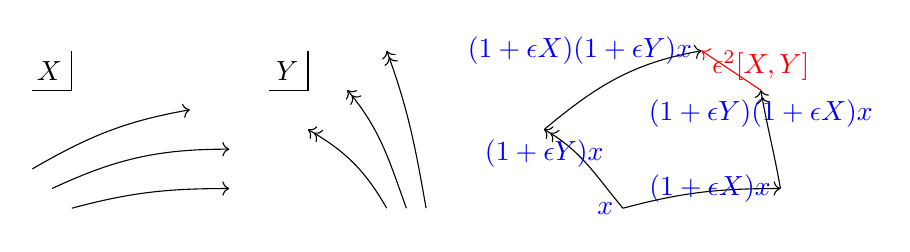
\begin{tikzpicture}
    \draw (0.5,1.5)--(1,1.5)node[above left]{$X$}--(1,2);
    
    \draw[->] (0.5,0.5) to [out=30,in=-170] (2.5,1.25);
    \draw[->] (0.75,0.25) to [out=25,in=-180] (3,0.75);
    \draw[->] (1,0) to [out=15,in=-180] (3,0.25);
    
    \draw (3.5,1.5)--(4,1.5)node[above left]{$Y$}--(4,2);
    
    \draw[<<-] (5,2) to [out=-70,in=100] (5.5,0);
    \draw[<<-] (4.5,1.5) to [out=-50,in=110] (5.25,0);
    \draw[<<-] (4,1) to [out=-30,in=120] (5,0);
    
    \draw[->>] (8,0)node[blue,left]{$x$} to [out=130,in=-30] (7,1)node[blue,below]{$(1+\epsilon Y)x$};
    \draw[->] (8,0) to [out=15,in=-180] (10,0.25)node[blue,left]{$(1+\epsilon X)x$};
    \draw[->>] (10,0.25) to [out=100,in=-80] (9.75,1.5)node[blue,below]{$(1+\epsilon Y)(1+\epsilon X)x$};
    \draw[->] (7,1) to [out=40,in=-170] (9,2)node[blue,left]{$(1+\epsilon X)(1+\epsilon Y)x$};
    \draw[red,->] (9.75,1.5)node[above]{$\epsilon^2[X,Y]$}--(9,2);
\end{tikzpicture}\]
まず、$[X,Y]$とは、$X,Y$の非可換性を表す量であった。時刻0で$x$を通る$X$の積分曲線の時刻$\epsilon$での点を$(1+\epsilon X)x$と書く(悪い書き方だが)と、$(1+\epsilon X)(1+\epsilon Y)x$と$(1+\epsilon Y)(1+\epsilon X)x$は一般には一致せず、その差がだいたい$\epsilon^2[X,Y]_x$くらいになる。\\
積分曲線とはベクトル場の矢印をなぞって曲線を描く操作だったのと同様、積分多様体とは$D_p$という微小な正方形をペタペタ貼り合わせていく操作となる。このとき貼り合わせていく順番が問題となる。\\
まず、$X\subset D$に対し$D_x$を$D_{(1+\epsilon X)x}$に動かす操作は「スライド」するだけで「上下方向のズレ」は生じない(これは$X_x\in D_x$だから)。つまり、$D_x$と$D_{(1+\epsilon X)x}$は貼り合わされるべきである。\\
故に$X,Y\subset D$のとき$D_x,D_{(1+\epsilon X)x},D_{(1+\epsilon Y)x},D_{(1+\epsilon X)(1+\epsilon Y)x},D_{(1+\epsilon Y)(1+\epsilon X)x}$は貼り合っていて、$D_{(1+\epsilon X)(1+\epsilon Y)x}$と$D_{(1+\epsilon Y)(1+\epsilon X)x}$に上下方向のズレはないから、さっきの議論とは逆に$\epsilon^2[X,Y]_x\in D_x$となる。これは「積分多様体があれば包合的」を意味するが、逆に包合的であれば微小な正方形を貼り合わせていく順番に依存しないから積分多様体を構成することができる。
\begin{lem}[$\phi$-related]\label{lem:121}
    $\phi:M\to N$と$M,N$上のベクトル場$X',X$について
    \[(X,X')\text{が}\phi\text{-related}\overset{def}{\iff}\forall p\in P\ d\phi(X'_p)=X_{\phi(p)}\]
    このとき $(X,X')$と$(Y,Y')$が$\phi$-relatedならば$([X,Y],[X',Y'])$も$\phi$-related。
\end{lem}
\begin{proof}
    $d\phi(X'_p)$の微分作用素としての実体は $d\phi(X'_p)f:=X'_p(f\circ\phi)$ であった。つまり$\phi$-relatedの条件は「全ての$M$上の関数$f$で$\forall p\in P\ X'_p(f\circ\phi)=X_{\phi(p)}f$」、即ち$X'(f\circ\phi)=(Xf)\circ\phi$ということである。
    \begin{align*}
        [X',Y'](f\circ\phi)&=X'Y'(f\circ\phi)-Y'X'(f\circ\phi)\\
        &=X'((Yf)\circ\phi)-Y'((Xf)\circ\phi)\\
        &=(XYf)\circ\phi-(YXf)\circ\phi\\
        &=([X,Y]f)\circ\phi
    \end{align*}
\end{proof}
まず次を示す。
\begin{thm}[Frobeniusの定理(前半)]\label{thm:122}
    分布$D$に各$m\in M$を通る積分多様体が存在するならば$D$は包合的。
\end{thm}
\begin{proof}
    $m\in M$に対し$\iota:P\hookrightarrow M,\ m\in\iota(P)$を取る。\\
    $X,Y\subset D$に対し$X_{\iota(p)},Y_{\iota(p)}\in D_{\iota(p)}=d\iota(P_p)$だから$X_{\iota(p)}=d\iota(X'_p),Y_{\iota(p)}=d\iota(Y'_p)$となる$X'_p,Y'_p\in P_p$が各$p\in P$で取れるが、$\iota$は局所的には$\R^c\subset\R^d$だから$X',Y'$は$C^\infty$級であり、ベクトル場になる。\\
    $(X,X'),(Y,Y')$は$\iota$-relatedになるよう定められたから、先の補題から$([X,Y],[X',Y'])$も$\iota$-related、\\
    つまり$[X,Y]_{\iota(p)}=d\iota([X',Y']_p)\in d\iota(P_p)=D_{\iota(p)}$ となる。これが全ての$m\in M$で成立するから$[X,Y]\subset D$となる。
\end{proof}
逆向きを示す準備として次の補題を示す。
\begin{lem}
    $M$上のベクトル場$X$と$m\in M$に対し$X_m\neq0$なら$m$の局所座標$(U,\tau)$で$\tau_*X=\pdiff{}{x_1}$とできる。
\end{lem}
\begin{proof}
    $m$を通る超曲面$S$を$X_m\notin S_m\subset M_m$と取る。つまり$S_m+\R X_m=M_m$となる。\\
    \[\Phi:(-\epsilon,\epsilon)\times S\ni(t,x)\longmapsto(1+t X)x\in M\]
    と定める。このとき $\pdiff{}{t}\Phi(t,x)=X_x,\ \pdiff{}{x_i}\Phi(0,x)=\pdiff{}{x_i}$ となる。つまり、$d\Phi_{(0,m)}:\R\times S_m\to M_m$は
    \[d\Phi_{(0,m)}=\bordermatrix{
        & \color{blue}\R & \color{blue}S_m\cr
        \color{blue}M_m & X_m & \id_{S_m}\cr
    }\]
    となり、正則行列。$\tau:=\Phi^{-1}$とすれば、$\Phi_*\pdiff{}{t}=X$ だから$\tau_*X=\pdiff{}{t}$となる。
\end{proof}
\begin{thm}[Frobeniusの定理(後半)]\label{thm:123}
    包合的な$D$と$m\in M$に対し、次を満たす$m$の局所座標$(U,\tau)$が存在する。
    \[\tau_* D=\spn\left\{\pdiff{}{x_1},\dots,\pdiff{}{x_c}\right\}\]
    別の言い方をすれば、$\forall a\in\R^{d-c}$に対し$S_a:=\tau^{-1}(\R^c\times\{a\})$が$D$の積分多様体となる。
    また、$U$に含まれる連結積分多様体は上のあるスライス$S_a$に含まれる。
\end{thm}
\begin{proof}
    「任意の多様体$M$とその上の$c$次元包合的分布$D$について主張が成立」という命題を$c$についての帰納法で示す。まず、$D$の局所的な基底$\{X_1,\dots,X_c\}$を取って、$X_1=\pdiff{}{x_1}$となる局所座標を取る。必要ならば$X_i\mapsto X_i-X_i(x_1)X_1\ (i=2,\dots,c)$とすれば$X_i(x_1)=0\ (i=2,\dots,c)$とできる。\\
    $S:=\{x_1=0\}$とすると、定理\ref{thm:122}の証明中と同じ理由により、$X_2,\dots,X_c$は$S$上のベクトル場$X'_2,\dots,X'_c$だと思える($S_m=\ker(dx_1)$に注意)。$D'_s:=\spn\{(X'_2)_s,\dots,(X'_c)_s\}$という$S$上の分布を平行化
    \[D'=\spn\left\{\pdiff{}{x_2},\dots,\pdiff{}{x_c}\right\}\]
    する$S$の座標を取り、合わせて$x_1,\dots,x_c$という$M$の局所座標を考える。このとき、まず$M$上で$X_1=\pdiff{}{x_1}$である。$S$上で$\spn\{(X'_2)_s,\dots,(X'_c)_s\}=\spn\{\pdiff{}{x_2},\dots,\pdiff{}{x_c}\}$ となっているが、$S_t:=\{x_1=t\}$上でもそうなっているかは非自明であり、ここが証明のメインステップである。緑のズレが0なことを言いたい。
    
    \[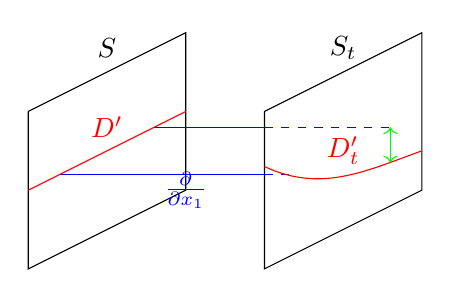
\begin{tikzpicture}
    \draw (0,2)--(0,0)--(2,1)--(2,3)--(0,2);
    \draw (3,2)--(3,0)--(5,1)--(5,3)--(3,2);
    \draw (1,2.8)node{$S$};
    \draw (4,2.8)node{$S_t$};
    
    \draw[blue] (0.4,1.2)--(3,1.2);
    \draw[blue,dashed] (3,1.2)--(3.4,1.2);
    \draw[blue] (1.6,1.8)--(3,1.8);
    \draw[blue,dashed] (3,1.8)--(4.6,1.8);
    \draw[blue] (2,1)node{$\pdiff{}{x_1}$};
    
    \draw[red] (0,1)--(2,2);
    \draw[red] (3,1.3) to [out=-25,in=200] (5,1.5);
    \draw[red] (1,1.8)node{$D'$};
    \draw[red] (4,1.5)node{$D'_t$};
    
    \draw[green][<->](4.6,1.8)--(4.6,1.35);
\end{tikzpicture}\]
    
    $[X_1,X_i]=\sum_{j=1}^c a_i^j X_j\ (i=2,\dots,c)$とすると、$l\geq c+1$に対して
    \[\pdiff{}{x_1}(X_i(x_l))=[X_1,X_l](x_l)=\sum_{j=2}^c a_i^j X_j(x_l)\]
    である、$X_1(x_l)=0$に注意。すると、これは$\{X_i(x_l)\}_i$という$c-1$個の未知変数についての線形常微分方程式をなし、$x_1=0$では初期値$0$を持つ($S$上では揃っている!)から$M$上で$X_i(x_l)=0$となる。つまり\\
    \[D_m\subset\set{v\in M_m}{\forall l\geq c+1\ v(x_l)=0}=\spn\left\{\pdiff{}{x_1},\dots,\pdiff{}{x_c}\right\}\]
    となるが、次元が等しいから上の包含は等号である。\\
    逆に、$\iota(P)\subset U$となる連結積分多様体$\iota:P\hookrightarrow M$について、$\iota(P)\subset\R^c\times\{{}^\exists a\}$となることを見る。それには$\pi:\R^d\to\R^{d-c}$について$\pi\circ\iota$が定数関数になればよく、その微分が消えるからOK。
    \[d(\pi\circ\iota)(P_p)=\pi(d\iota(P_p))=\pi(D_{\iota(p)})=0\]
\end{proof}


\ \\
\subsection{極大積分多様体}
\begin{lem}[積分多様体の位相]
    $\iota:P\hookrightarrow M$を$D$の積分多様体とする。このとき定理\ref{thm:123}でのスライス$S_a$について、任意の$U,a$に対し$\iota^{-1}(S_a)\subset P$が開になる。また、$\iota:\iota^{-1}(S_a)\to S_a\cap\iota(P)$は同相になる。
\end{lem}
\begin{proof}
    $p\in P$と$m:=\iota(p)$の近傍$U_p,U_m$を$\iota(U_p)\subset U_m$かつ$U_p$が連結となるように取る。$\iota:U_p\hookrightarrow M$も積分多様体だから、$\exists a\ \iota(U_p)\subset S_a$となる。つまり、$a\in\R^{d-c}$に対し$\iota^{-1}(S_a)$は$\supset U_p$か$=\emptyset$となる。これが全ての$p\in P$について成り立つから$\iota^{-1}(S_a)$は開になる。同相性は$\iota:\iota^{-1}(S_a)\to S_a$が同じ次元のはめ込み($\Rightarrow$開写像)になるため。
\end{proof}

\begin{thm}[命題\ref{prop:111}を参照]\label{thm131}
    $\phi:N\to M$が$\phi(N)\subset\iota(P)$を満たすとき、$\phi_0:N\to P$は連続。従って$C^\infty$級。
    \[\begin{tikzcd}
        N\arrow[rd,"\exists \phi_0"']\arrow[r,"\phi"] &M\\
        & P\arrow[u,hook]
    \end{tikzcd}\]
\end{thm}
\begin{proof}
    先の補題とほぼ同様である。$p:=\phi_0(n),m:=\iota(p),\ \phi(U_n)\subset U_m$と十分小さく近傍を取る。$U_n$を予め連結にしておく。$U_m\cap\iota(P)$の連結成分の個数は第二可算性から高々可算であり、各成分はあるスライスに入るから、結局$U_m\cap\iota(P)$は可算枚のスライスに含まれる。$\phi(U_n)\subset U_m\cap\iota(P)$は連結部分集合だから、$\phi(U_n)$はあるスライス$S_a$に含まれる。$\phi_0(U_n)\subset\iota^{-1}(S_a)$であり、前補題から$\iota^{-1}(S_a)\cap U_m$は$p$の近傍系をなすから$\phi_0$は$n$で連続。
\end{proof}
\begin{thm}[極大積分多様体]
    $D$を包含的とすると、$\forall m\in M$に対し$m$を通る極大積分多様体$\iota:P\hookrightarrow M$が存在する。つまり、$P$は連結であり、$\iota':P'\hookrightarrow M$を$m$を通る連結な積分多様体とすると$\iota'(P')\subset\iota(P)$となる(最大性)。
\end{thm}
\begin{proof}
    次は、「$U\subset M$が開$\overset{def}{\iff}\forall i\ \tau_i(U\cap U_i)\subset\R^n$が開」で位相が定まると思えばよい。このとき、$\tau_i:U_i\to\R^n$が同相になることを確かめればよい($U_i$には$M$からの相対位相が入っている)。
    \begin{rem}[多様体の定義]
        集合$M$を被覆する部分集合族$\{U_i\}_i$と全単射の族$\tau_i:U_i\to\R^n$が与えられたとき、次の条件を満たせば$M$は$\{\tau_i:U_i\to\R^n\}$をアトラスとする多様体構造が定まる。
        \begin{itemize}
            \item $\tau_j(U_i\cap U_j)$は開集合かつ、$\tau_j\circ\tau_i^{-1}:\tau_i(U_i\cap U_j)\to\tau_j(U_i\cap U_j)$は$C^\infty$級。
        \end{itemize}
    \end{rem}
    多様体$\Tilde{M}$を、集合としては$M$だが、アトラスとして次の写像の族$\{\tau_i:U_i\to\R^c\}$を持つものとする。
    \[\tau_i:U_i:=\tau^{-1}(\R^c\times\{a\})\overset{\tau}{\longrightarrow}\R^d\twoheadrightarrow\R^c\]
    ただし記号は定理\ref{thm:123}の通りであり、上の写像は可能な全ての$(U,\tau),a$で考える。これが上の注意の条件を満たすことを確かめる。$\tau_i(U_i\cap U_j)$が開であれば残りは自動的である。なぜなら、まず$U_i$は$\tau_i$を座標に持つ$M$の部分多様体であり、$\tau_i(U_i\cap U_j)$が開だから$U_i\cap U_j$も部分多様体になる。二つの座標$\tau_i,\tau_j$の座標変換は当然$C^\infty$級となる。\\
    今、$U_i=\tau^{-1}(\R^c\times\{a\}),\ U_j=\tau'^{-1}(\R^c\times\{a'\})$と、$(U,\tau,a)$と$(U',\tau',a')$から作られているとする。$U_j$は$D$の積分多様体だから$U\cap U_j$の各連結成分は$\tau^{-1}(\R^c\cap\{a"\})$という形の部分集合にスッポリ入っている。$U\cap U_j$の連結成分は$U_j$内で開だから、その合併である$U_i\cap U_j$も$U_j$内で開。$\tau_j$は同相だから$\tau_j(U_i\cap U_j)\subset\R^n$も開。\\
    \ \\
    上で作った$\Tilde{M}$での$m$の連結成分$P$には$\Tilde{M}$からの多様体構造が入る。示すべきは二つである:$P$の第二可算性と最大性。後者の方が簡単なのでそっちから片す。\\
    $\iota':P'\hookrightarrow M$を積分多様体とすると、$\iota':P'\hookrightarrow \Tilde{M}$も連続になる。これは$\iota'^{-1}(S_a)\subset P$が開であることから従う。故に$\iota'(P')\subset\Tilde{M}$は連結であり、$\iota'(P)\subset P$となる。\\
    $\Tilde{M}$のアトラスとして与えた$\{U_i\}$が「$\forall i\ \abs{\set{j}{U_j\cap U_i\neq\emptyset}}\leq\abs{\N}$」を満たすことを見ればいい。なぜなら「交わるかどうか」で添字集合にグラフ構造が入るが、各頂点の次数は高々可算だからグラフの各連結成分の頂点数も高々可算となり、グラフの連結成分への分解に応じて$\Tilde{M}$も開集合の非交和に分解される。つまり$P$が高々可算枚のアトラスで覆えることになり第二可算性が従う。\\
    $U_i$は全ての$(U,\tau),a$について考えると書いたが、少し変えて、$M$の第二可算性から$(U,\tau)$は可算枚で事足りるのでそうする。$U_i=\tau^{-1}(\R^c\times\{a\}),U_j=\tau'^{-1}(\R^c\times\{a'\})$と書くと、$U_i\cap U'$の連結成分は高々可算個だから、各$U'$について$U_i\cap U_j\neq\emptyset$となる$a'$も高々可算個の可能性しかない。可算×可算で$j$も高々可算個。
\end{proof}

\subsection{Cartanの方法}
$M,N$を多様体とする。各点$(m,n)\in M\times N$に対し、$\phi_{m,n}:M_m\to N_n$という線形写像の族が$m,n$に対し滑らかに与えられたとする。このとき、$\phi:M\to N$であって$\forall m\in M\ d\phi_m=\phi_{m,\phi(m)}$となるものが存在するか?という問が考えられる。
\[D_{(m,n)}:=\phi_{m,n}\text{のグラフ}:=\set{(v,\phi_{m,n}v)}{v\in M_m}\]
という分布がもし包合的ならば、Frobeniusの定理から極大積分多様体$\iota:P\hookrightarrow M\times N$が存在し
\[d\iota(P_p)=\phi_{\iota(p)}\text{のグラフ}\]
となる。故に、$P\hookrightarrow M\times N\to M$は同じ次元の多様体の間のはめ込みである。特に局所微分同相であり、つまり局所的には所望の写像$\phi:M\to N$が存在することになる。
\newpage
\section{Lie群}


\subsection{Lie群とLie環の対応}
\begin{defi}[Lie群]
    多様体$G$が群構造を持っていて演算が全て$C^\infty$級のときLie群と呼ぶ。$C^\infty$な群準同型を単にLie群の準同型と呼ぶ。\\
	部分多様体$H\hookrightarrow G$がLie群の準同型であるとき部分Lie群と呼ぶ\footnotemark。つまり、部分群でも部分多様体でもありそれ自身Lie群になるもの。
\end{defi}
\footnotetext{後に示すこととして、この定義と「部分多様体化可能な部分群」は同等。}
\begin{eg}
    \begin{itemize}
        \item 可換な例。$G=\R^n\times\T^m$。はめ込まれた部分多様体の典型例として、$\T^2$内での「ぐるぐるするやつ」があるが、これは部分Lie群である。しかし閉ではない。
        \item $GL(n,\R)$とか。線形群。
        \item アフィン変換群、または$\R_{>0}$と$\R$の半直積。つまり、多様体としては$G=\R_{>0}\times\R$だが
        \[(s,t)(s',t'):=(ss',st'+t)\]
        で群構造を入れたもの。一番簡単な非可換Lie群でありnon unimodular。
    \end{itemize}
\end{eg}

\begin{defi}[Lie環]
    $\g$が有限次元$\R$-線形空間で次を満たす双線形写像$[,]:\g\times\g\to\g$を備えているとき、Lie環と呼ぶ。
    \[[X,Y]=-[Y,X],\ [X,[Y,Z]]+[Y,[Z,X]]+[Z,[X,Y]]=0\]
    線形であって括弧を保つものをLie環の準同型と呼ぶ。\\
    括弧で閉じた部分線形空間を部分Lie環と呼ぶ。
\end{defi}
\begin{eg}
    \begin{itemize}
        \item 可換な例。$\g:=V$に$[X,Y]:=0$で括弧を入れたもの。
        \item $\g:=M(n,\R)$に$[X,Y]:=XY-YX$で括弧を入れたもの。一般に結合的多元環は同じ構成でLie環と見做せる。
        \item $\g:=\spn\{X,Y\}$に$[X,Y]:=Y$で括弧を入れたもの。
    \end{itemize}
\end{eg}


\begin{defi}[平行移動]
    左移動を$L_y:G\ni x\mapsto yx\in G$と定める。また、$\g$をその左不変ベクトル場全体と定める:
    \[\g:=\set{X\in\X(G)}{\forall y\in G\ (L_y)_*X=X}\]
\end{defi}
\begin{prop}
    \[\g\ni X\longmapsto X_e\in G_e\]
    は線形同型である。また、$\X(G)$の括弧積について$\g$は閉じていて、故に$\g$はLie環となる。
\end{prop}
\begin{proof}
    $X_x=dL_x(X_e)$より単射性は明らか。逆に、$v\in G_e$について$X_x:=dL_x(v)$と構成すれば$X_e=v$だが、$X$の$C^\infty$級性がやや非自明である。$f\in C^\infty(G)$に対し$Xf\in C^\infty(G)$を示せば十分だが、
    \[(Xf)_x=v(f\circ L_x)=\sum_i a_i\pdiff{}{y_i}f(xy),\ v=\sum_i a_i\pdiff{}{y_i}\]
    だから、$f(xy)$という$G\times G$上の関数の$C^\infty$級性から降ってくる。\\
    $X\in\g$は$X$が自分自身と$L{{}^\forall y}$-relatedであることと同値、故に$\g$は補題\ref{lem:121}から括弧積で閉じている。$\X(G)$の括弧積は反対称性やJocobi律を満たす($\mathrm{End}(C^\infty(G))$は結合的だから!)ので$\g$はLie環になる。
\end{proof}
\begin{defi}[Lie群に対応するLie環]
    左不変ベクトル場$\g$、または単位元の接空間$G_e$を付随するLie環と呼ぶ。
\end{defi}

\begin{eg}
    \begin{itemize}
        \item $G=\R^n\times\T^m$に対し$\g=\R^{n+m}$は可換なLie環。
        \item $G=\mathrm{GL}(n,\R)$に対し$\g=\mathrm{M}(n,\R)$となる。
        \item $G=\R_{>0}\ltimes\R$に対し$\g=\spn\{X,Y\},\ [X,Y]:=Y$となる。
    \end{itemize}
\end{eg}
関手性と忠実性を説明するために少し準備をする。
\begin{thm}[関手性]
    準同型$\phi:G\to H$に対し、$\phi_*:\g\cong G_e\overset{d\phi}{\longrightarrow}H_e\cong\h$はLie環の準同型。
\end{thm}
\begin{proof}
    つまり$\phi_*X$とは、$d\phi(X_e)\in H_e$を平行移動させてできるベクトル場である。まず、$X,\phi_*X$が$\phi$-relatedであることを見る。$x\in G$に対して$d\phi(X_x)\overset{?}{=}(\phi_*X)_{\phi(x)}$を見ればよいが、$L_{\phi(x)}\circ\phi=\phi\circ L_x$より
    \[(\phi_*X)_{\phi(x)}:=dL_{\phi(x)}d\phi(X_e)=d\phi dL_xX_e=d\phi X_x\]
    となってOK。\\
    補題\ref{lem:121}より、$[X,Y],[\phi_*X,\phi_*Y]$が$\phi$-relatedである。ある左不変ベクトル場と$\phi$-relatedな左不変ベクトル場は一意的(原点での値だけで決まる!)だから、$\phi_*$が括弧と交換する。
\end{proof}


\begin{thm}[部分群と部分環の対応]\label{thm:311}
    連結Lie群$G$を固定する。次の対応は互いに逆。
    \[\begin{array}{ccc}
        \set{\iota:H\hookrightarrow G}{\text{連結部分Lie群}} & \longleftrightarrow & \set{\h\subset\g}{\text{部分Lie環}}\\
        H & \longmapsto & \iota_*(\h)\\
        \text{積分多様体} & \longmapsfrom & \h
    \end{array}\]
\end{thm}
\begin{proof}
    まず、$\iota_*$がLie環の準同型だからその像$\iota_*(\h)$は部分Lie環である。$\h\subset\g$に対し
    \[D_x:=\set{X_x}{X\in\h}\]
    で定まる左不変な分布が包合的であることは、注意\ref{rem:121}より$\h$が括弧積で閉じていることから従う。故に$e\in G$を含むその極大積分多様体$H$が取れるが、$H\subset G$が部分群であることと積分多様体としての微分構造について演算が全て滑らかになることを見る。\\
    $dL_y(D_x)=D_{yx}$の意味で左不変だから、$L_y(H)$も同じ分布の極大積分多様体である。両辺$e$を含むから、$x\in H$に対し$L_{x^{-1}}H=H$となり、$H\subset G$は部分群。
	故に、演算の制限$H\times H\to G$は$H$を経由するから、定理\ref{thm131}から$H$自身Lie群になる。
	\[\begin{tikzcd}
	    H\times H\arrow[rd,"\exists!"']\arrow[r]& G\\
	    & H\arrow[u,hook]
	\end{tikzcd}\]
	$\mapsfromup=\id$は作り方からOK。$H\subset G$に対し、$\mapstodown$をしてできる極大積分多様体$H'$との一致を見る。$H\hookrightarrow G$自体も同じ分布に対する積分多様体(原点でそう!)だから最大性から
	\[\begin{tikzcd}
	    H\arrow[rd,"\exists!"']\arrow[r]& G\\
	    & H'\arrow[u,hook]
	\end{tikzcd}\]
	であるが、$\phi:H\to H'$は同じ次元の多様体間の単射はめ込みであり、$\phi(H)\subset H'$は開部分群である。$H'$の連結性から$\phi(H)=H'$であり、つまり$\phi$はLie群の同型。
\end{proof}

この定理を準同型のグラフに用いることで次のような命題を得る。
\begin{prop}\label{prop:311}
    連結Lie群$G,H$とそのLie環の準同型$\Phi:\g\to\h$が与えられたとする。$G$が単連結ならLie群の準同型$\phi:G\to H$で$\phi_*=\Phi$となるものが存在し、一意。
\end{prop}
\begin{proof}
    $G\times H$というLie群に対応するLie環は$\g\times\h$であり、$\Phi$のグラフは$\g\times\h$の部分Lie環である。故に前定理から$G\times H$の部分Lie群$G'$であって
    \[\forall(x,y)\in G'\ \ \ G'_{(x,y)}=\set{(X,\Phi(X))}{X\in\g}\subset G_x\times H_y\]
    となるものが存在する。$G$成分への射影の制限$p:G'\hookrightarrow G\times H\twoheadrightarrow G$ がLie群の同型であることがもし言えたなら、$\phi:G\overset{p^{-1}}{\longrightarrow}G'\hookrightarrow G\times H\twoheadrightarrow H$はLie群の準同型であり$\phi_*=\Phi$を満たす。\\
    $dp:G_e\to G'_e$は$dp(v)=(v,\Phi(v))$だから線形同型であり、準同型性から各点で微分が線形同型なので$p:G'\to G$は局所微分同相となる。開写像性から$p(G')\subset G$が開部分群(つまり開かつ閉)となり、$G$の連結性から$p$は全射。また、$\Gamma:=\ker p$は単位元での局所微分同相性から、単位元の開近傍$U\subset G'$であって
    \[\forall s\neq t\in\Gamma\ \ \ sU\cap tU=\emptyset\]
    となるものが取れ、$p(U)$の平行移動がevenly coveredな$G$の開被覆を与えるから$p$は被覆。単連結性から$p$は全単射となる。局所微分同相性と準同型性と合わせれば、$p$がLie群の同型になることが分かる。\\
    一意性は、$\psi_*=\Phi$となる準同型$\psi:G\to H$のグラフが$G\times H$の部分Lie群であって、対応する$\g\times\h$の部分Lie群が$\Phi$のグラフであることから従う。
\end{proof}

\begin{prop}
    連結Lie群$G$の被覆空間$p:\Tilde{G}\to G$には$p$が局所微分同相かつ群準同型となるようなLie群の構造が入る。特に、$G$の普遍被覆は単連結Lie群となる。
\end{prop}
\begin{proof}
    $p$が微分同相となるような$\Tilde{G}$上の$C^\infty$級構造は一意で、$G$内のevenly coveredな局所座標を持ち上げたもの全体が$\Tilde{G}$のアトラスとなる。$\Tilde{e}\in p^{-1}(e)$を一つ選ぶと、それに応じて$p$が群準同型となるように$\Tilde{G}$にLie群の構造が入って一意的であることを確認する。
    \begin{fact}[lifting property(強)]
        基点付き空間$(X,x_0),(\Tilde{X},\Tilde{x}_0),(Y,y_0)$とその間に基点を保つ連続写像$f:(Y,y_0)\to(X,x_0),p:(\Tilde{X},\Tilde{x}_0)\to(X,x_0)$が与えられたとする。$p$が被覆で$f$が
        \[f_*(\pi_1(Y,y_0))\subset p_*(\pi_1(\Tilde{X},\Tilde{x}_0))\]
        を満たすなら、連続写像$\Tilde{f}:(Y,y_0)\to(\Tilde{X},\Tilde{x}_0)$であって$p\circ\Tilde{f}=f$なるものが存在し一意。
        \[\begin{tikzcd}
            & (\Tilde{X},\Tilde{x}_0)\arrow[d,"p"]\\
            (Y,y_0)\arrow[ru,"\Tilde{f}"]\arrow[r,"f"] & (X,x_0)
        \end{tikzcd}\]
    \end{fact}
    \[F:(G\times G,(e,e))\ni (x,y)\longmapsto x^{-1}y\in (G,e)\]
    と置き、$f:=F\circ(p\times p)\ :(\Tilde{G}\times\Tilde{G},(\Tilde{e},\Tilde{e}))\to(G,e)$ について考える。
    \begin{fact}[位相群の基本群は可換]
        $[c],[d]\in\pi_1(G,e)$の積として、各点毎で$G$の演算を行なったもの$[c\times d]$とループの結合$[c\dot d]$がある
        \[(c\times d)(t):=c(t)d(t),\ \ \ (c\dot d)(t):=\begin{cases}
            t\leq\frac12 & c(2t)\\
            t\geq\frac12 & d(2t-1)
        \end{cases}\]
        が、これらはホモトピックである。
    \end{fact}
    から、$F_*([c],[d])=[c^{-1}\times d]=[c]^{-1}[d]$は基本群のレベルでも$F_*(\alpha,\beta)=\alpha^{-1}\beta$という準同型になる。\\
    故に$p_*\pi_1(\Tilde{G},\Tilde{e})\subset\pi_1(G,e)$が部分群であることから、lifting propertyの仮定が満たされる。
    \[\begin{tikzcd}
        \Tilde{G}\times\Tilde{G}\arrow[r,"\Tilde{f}"]\arrow[d,"p\times p"'] &\Tilde{G}\arrow[d,"p"]\\
        G\times G\arrow[r,"f"] & G
    \end{tikzcd}\]
    群の公理は$f:G\times G\ni(x,y)\mapsto x^{-1}y\in G$と$e\in G$の言葉だけで書けるが、lifting propertyの一意性から、$G$での群の公理が$\Tilde{G}$上でも成立することが分かる。また、$\Tilde{f}$には連続性しかないが、$p$は局所微分同相なので$\Tilde{f}$は$C^\infty$級。即ち$\Tilde{G}$はLie群となる。
\end{proof}
以上をまとめると、次になる。
\begin{thm}[単連結Lie群とLie環の対応]
    \[G\longmapsto\g,\ \ \ \hom(G,H)\ni\phi\longmapsto\phi_*\in\hom(\g,\h)\]
    は単連結Lie群のなす圏とLie環のなす圏の圏同値を与える。
\end{thm}
\begin{proof}
    忠実充満性、即ち$\hom(G,H)\ni\phi\mapsto\phi_*\in\hom(\g,\h)$の全単射性は命題\ref{prop:311}で既に示した。本質的全射性は次の代数的な事実から分かる。
    \begin{fact}[Adoの定理]
        全てのLie環は行列環のなすLie環の部分Lie環として実現できる。\\
        参照:\url{https://terrytao.wordpress.com/2011/05/10/ados-theorem/}
    \end{fact}
    部分Lie群と部分Lie環の対応から、Lie環$\g$に対応するLie群$G$は$\mathrm{GL}(n,\R)$の部分群として構成できる。更にその普遍被覆$\Tilde{G}$を取れば、$\Tilde{G}$のLie環と$\g$は同型である。なぜなら、左不変ベクトル場が自然に持ち上がり、局所微分同相性より括弧積が保たれるから。
\end{proof}
\begin{prop}
    普遍被覆を取る関手$G\longmapsto\Tilde{G}$は忠実かつ本質的全射。つまり、
    Lie群の準同型$\phi:G\to H$は一意的に普遍被覆に持ち上がる。より詳しく言えば、次の準同型$\Tilde{\phi}$は存在し一意:
    \[\begin{tikzcd}
        \Tilde{G}\arrow[r,"\Tilde{\phi}"]\arrow[d,"p"'] &\Tilde{H}\arrow[d,"p"]\\
        G\arrow[r,"\phi"] & H
    \end{tikzcd}\]
\end{prop}
\begin{proof}
    本質的全射は単連結な部分圏に制限して$\id$だから明らか。関手性は一意性から出てくるので、$\Tilde{\phi}$の一意性を言えばいいが、lifting propertyから直ちに出る。
\end{proof}
例えば、Lie環が同型であることと同型な普遍被覆を持つことが同値だったり、$\hom(G,H)\ni\phi\longmapsto\phi_*\in\hom(\g,\h)$が一般に単射\footnotetext{Lie環の準同型が全てLie群の準同型に持ち上がるわけではないが、少なくとも局所的には準同型になるため、そういったものを局所準同型と呼ぶことがある。}であることが分かる。Lie群は「そのLie環と基本群」の情報だけで同型類を記述することができ、こういうノリがLie群Lie環対応である。\\
\ \\
Lieの第三定理(Lie群Lie環対応の本質的全射性)をAdoの定理を経由せずに示す方法を知ったので追記。
\begin{thm}[Lieの第三定理]
    任意のLie環$\g$はある(単連結)Lie群$G$のLie環と同型になる。
\end{thm}
\begin{proof}
    $\g$の中心を$C$、$\g/C$を$\Tilde{\g}$と書く。$\Tilde{\g}$は随伴表現により$End(\g)$に埋め込むことができるが、$End(\g)$はあるLie群のLie環であることが既に分かっているから、$\Tilde{\g}$は単連結Lie群$\Tilde{G}$のLie環として実現できる。\\
    次の事実だけ認める。
    \begin{fact}
        Lie群の2次ホモトピー群は常に0。
    \end{fact}
    Hurewiczの定理から$\Tilde{G}$の2次以下のホモロジー群$H_1(G),H_2(G)=0$であり、普遍係数定理とde Rhamの定理から$\Tilde{G}$の2次以下の「$C$値de Rhamコホモロジー」も消える。
    \[0\to C\to \g\to\Tilde{\g}\]
    という拡大があるので、(線形空間のレベルでの)セクション$s:\Tilde{\g}\to\g$を取って
    \[\Psi(X,Y):=[s(X),s(Y)]-s([X,Y])\ \ \ (X,Y\in\Tilde{\g})\]
    という、$\Psi:\Tilde{\g}\times\Tilde{\g}\to C$が定まる。Lie環の公理から$\Psi$は反対称($\Psi(Y,X)=-\Psi(X,Y)$)であり
    \[\Psi([X,Y],Z)+\Psi([Z,X],Y)+\Psi([Y,Z],X)=0\]
    となる\footnote{これが群の拡大のときの2-cocycle条件に相当する?}。$\Psi\in\hom(\wedge^2\Tilde{\g},C)=C\otimes\wedge^2\Tilde{\g}^*=C\otimes\wedge^2 T^*_e\Tilde{G}$ と同一視して、平行移動で動かすことで$\Psi$は$\Tilde{G}$上の$C$値2次微分形式だと思える。外微分の内在的な表記(長い式)から、$\Psi([X,Y],Z)$の巡回和が0という条件は$d\Psi=0$と同値である。先の事実から$\Psi=d\alpha$なる$\Tilde{G}$上の$C$値1次微分形式$\alpha$(左不変とは限らない)が存在する、完全1形式を引くことで$\alpha_e=0$としておく。\\
    $\Psi$の左不変性から$(L_g)^*\alpha-\alpha$は閉形式であり、$L_g^*\alpha-\alpha=df_g$かつ$f_g(e)=0$なる$f_g:\Tilde{G}\to C$が存在する。この$f_g$というのは($\Tilde{G}$の単連結性から)具体的に
    \[f_g(h)=\int_e^h (L_g^*\alpha-\alpha)\]
    と記述できるから、$F(g,h):=f_g(h)$は$F:\Tilde{G}\times\Tilde{G}\to C$という$C^\infty$級写像を定める。
    \begin{align*}
        L_{gh}^*\alpha-\alpha &= L_h^*(L_g^*\alpha-\alpha)+(L_h^*\alpha-\alpha)\\
        df_{gh} &= L_h^*df_g+df_h\\
        f_{gh} &= f_g\circ L_h + f_h +C\ \ \ \exists C=C_{g,h}\\
        F(gh,k)+F(g,h) &= F(g,hk)+F(h,k)
    \end{align*}
    定数$C$の特定に$F(-,e)=0$を使った。これにより$F$は2-cocycle条件を満たすので、$G:=\Tilde{G}\times C$上に
    \[(g,a)\times(h,b):=(gh,a+b+F(g,h))\]
    で群構造が入り、$G$には直積として微分構造が入る。$F$がそうだから演算は全て$C^\infty$級となる。\\
    残るは、元々のLie環$\g$と$G$のLie環の同型である。それは、セクション$s$による同一視$\g\cong\Tilde{\g}\times C$と$T_e G\cong T_e\Tilde{G}\times C$の合成によって得られることを確認する。まず、元のLie環の構造は$\Tilde{\g}\times C$に
    \[[(X,A),(Y,B)]:=[s(X)+A,s(Y)+B]=s[X,Y]+\Psi(X,Y)=([X,Y],\Psi(X,Y))\]
    で入る。また、$(X,A)\in T_e\Tilde{G}\times C$を平行移動したものは(積の定義から)
    \[L_{(g,a)}(X,A)=(dL_gX,A+df_gX)\]
    である。$G$上の左不変ベクトル場の第一成分は$\Tilde{G}$上の左不変ベクトル場であり、第二成分は$C$上の左不変ベクトル場に$\Tilde{G}$成分だけに依存するベクトル場を足したものとなる。$(X,A+df_g(X_e))\ \ X\in\g,A\in C$と書ける。特に、$G$上の左不変ベクトル場を$C$の方向に微分しても0である。
    \begin{align*}
        &[(X,A+df_g(X_e)),(Y,B+df_g(Y_e))]\\
        =& [X,Y]+[X,B+df_g(Y_e)]+[A+df_g(X_e),Y]+[A+df_g(X_e),B+df_g(Y_e)]\\
        =& [X,Y]+X(B+df_g(Y_e))-Y(A+df_g(X_e))\\
        =& [X,Y]+X(L_g^*\alpha-\alpha)(Y_e)-Y(L_g^*\alpha-\alpha)(X_e)\\
        =& [X,Y]+X(\alpha(Y)_g)-Y(\alpha(X)_g)\\
        =& [X,Y]+X\alpha(Y)-Y\alpha(X)
    \end{align*}
    ここで、
    \[\Psi(X,Y)=d\alpha(X,Y)=X\alpha(Y)-Y\alpha(X)-\alpha([X,Y])\]
    より、最後の式は
    \[[X,Y]+\Psi(X,Y)+\alpha([X,Y])=[X,Y]+\Psi(X,Y)+\alpha([X,Y])_g-\alpha([X,Y])_e=[X,Y]+\Psi(X,Y)+df_g([X,Y])\]
    ただし、$\alpha_e=0$を使った。
\end{proof}



\newpage
\subsection{指数写像}
Lie群$G$に対し、$\R$は単連結Lie群だから命題\ref{prop:311}から次は全単射:
\[\hom(\R,G)\ni\phi\longmapsto\phi_*\in\hom(\R,\g)\]
故に、$X\in\g$に対し$d\phi_X(\pdiff{}{t})=X$なる準同型$\phi_X:\R\to G$が一意的に存在する。一意性から$\phi_X(st)=\phi_{sX}(t)$が成り立つため、この同型を調べるためには次を見れば十分である:
\begin{defi}[指数写像]
    $X\in\g$に対し、$\exp(X)\in G$を$\exp(X):=\phi_X(1)$と定める。
\end{defi}
つまり、$\phi_X(t)=\exp(tX)$となっている。
\begin{thm}
    \begin{enumerate}[(1)]
        \item $\exp(tX)\exp(sX)=\exp((s+t)X),\ \exp(-X)=\exp(X)^{-1}$
        \item $\phi_X$は$X$の積分曲線
        \item $X\in\g$の時間発展$\Phi_X^t:G\to G$は$\Phi_X^t(x)=x\exp(tX)$
        \item $\exp:\g\to G$は$C^\infty$級であり、$d\exp:\g_0\to G_e$は$\id_{\g}$
    \end{enumerate}
\end{thm}
特に、左不変ベクトル場は自動的に完備(時間有限で爆発しない)である。
\begin{proof}
    (1)は$\phi_X(t)=\exp(tX)$から明らか。(2)は次から分かる。
    \[(d\phi_X)_t(\pdiff{}{t})=dL_{\phi_X(t)}(d\phi_X)_e(\pdiff{}{t})=dL_{\phi_X(t)}(X_e)=X_{\phi_X(t)}\]
    更に、$X$の左不変性から、積分曲線を左平行移動したものも積分曲線となって(3)が分かる。\\
    (4)は$\g_0$の曲線の同値類の代表元として$t\mapsto tX$を選べば、次のように計算できる。
    \[(d\exp)_0(X)=\pdiff{}{t}\lvert_{t=0}\exp(tX)=X_e\]
\end{proof}
\begin{thm}(捕鯨)
    Lie群の準同型$\phi:G\to H$に対し次は可換(特に、群の$\exp$は部分群の$\exp$と一致):
    \[\begin{tikzcd}
        G\arrow[r,"\phi"] & H\\
        \g\arrow[u,"\exp"]\arrow[r,"\phi_*"] &\h\arrow[u,"\exp"']
    \end{tikzcd}\]
\end{thm}
\begin{proof}
    \[\pdiff{}{t}\lvert_{t=0}\phi\circ\phi_X(t)=d\phi(X_e)=\phi_*(X)_e\]
    より、一意性から$\phi\circ\phi_X=\phi_{\phi_*X}$となる。
\end{proof}
\begin{prop}
    部分Lie群$H\leq G$と$X\in\g$に対し
    \[\exp({}^\forall tX)\in H\iff X\in\h\]
\end{prop}
\begin{proof}
    先の可換性を$\iota:H\hookrightarrow G$に使えば、$(\Leftarrow)$が出る。逆は、捕鯨より$\phi_X$は$H$を経由するから
    \[\begin{tikzcd}
        \R\arrow[r,"\phi_X"]\arrow[rd,"\exists\psi"'] & G\\
        & H\arrow[u,hook]
    \end{tikzcd}\]
    \[X=\left.\pdiff{}{t}\right\lvert_{t=0}\phi_X(t)=d\iota d\psi\left(\pdiff{}{t}\right)\in \im (d\iota)=\h\]
\end{proof}
\begin{eg}[$GL(n,\R)$の場合]
    $G=GL(n,\R)$の場合$\g=M(n,\R)$だが、指数写像$\exp$と行列の指数関数は一致する。これは行列の指数関数が積分曲線になっていることを級数の項別微分で確かめれば良い。
\end{eg}


\ \\
\subsection{連続準同型}
\begin{lem}
    連続群準同型$\phi:\R\to G$は自動的に$C^\infty$級。
\end{lem}
\begin{proof}
    \[\exp:\g\supset U\xrightarrow{\cong}\exp(U)\subset G\]
    が同相となる$0$の開近傍$U$を取る。十分小さい$t$で $\phi(t)=\exp({}^{\exists !} X(t))$ と$X(t)$を定めると、更に小さいところで
    \[\forall n\ \forall\epsilon\ \ -\epsilon<t\epsilon\Rightarrow X(nt)=nX(t)\]
    $X:=\lim_{N\to\infty}2^NX(2^{-N})$は十分大きい$N$で一定だから極限が存在する。$p\in\Q$に対し十分小さい$t$で$X(pt)=pX(t)$となるから
    \[\phi(p)=\phi(2^{-N}p)^{2^N}=\exp(2^NX(2^{-N}p))=\exp(pX)\]
    $\phi$の連続性から$\phi(t)=\exp(tX)\ (t\in\R)$である。
\end{proof}
\begin{lem}(捕鯨)
    積$m:G\times G\to G$の微分$dm:T_eG\times T_eG\to T_eG$は$(v,w)\mapsto v+w$である。
\end{lem}
\begin{proof}
    全微分を計算するためには偏微分を計算すればよく、それは$m(x,e)$を調べ$x$に関し微分するという手続きである。$m(x,e)=x$だから明らか。
\end{proof}
\begin{thm}
    連続群準同型$\phi:G\to H$は自動的に$C^\infty$級。
\end{thm}
LieGrpからTopGrpへの忘却関手が忠実充満であることを意味している。
\begin{proof}
    $X\in\g$に対し$\R\ni t\mapsto\phi(\exp(tX))\in H$は連続群準同型、従って滑らかである。$\g$の基底$X_1,\dots,X_n$に対し
    \[\begin{tikzcd}
        \R^n\ni(t_1,\dots,t_n)\arrow[r]\arrow[dr] &\exp(t_1X_1)\dots\exp(t_nX_n)\in G\arrow[d,"\phi"]\\
        &\prod_{i=1}^n\phi(\exp(t_iX_i))\in H
    \end{tikzcd}\]
    $\R^n\to H$が$C^\infty$級であり、逆関数定理から$\R^n\to G$が局所微分同相(捕鯨)だから$\phi$は単位元近傍で$C^\infty$級。平行移動をすれば$G$全域で$C^\infty$級。
\end{proof}
\begin{cor}
    位相群をLie群化する微分構造は高々一意。
\end{cor}
\begin{proof}
    極大アトラス$\A_1,\A_2$に対し、$\id:(G,\A_1)\to(G,\A_2)$とその逆は連続群準同型だから。
\end{proof}
ではLie群化可能な位相群はどういったクラスか?と言うと、実は局所Euclidな位相群に対しては必ずLie群化する微分構造が存在する。つまり、TopGrpのうち局所Euclidな位相群のなす部分圏へのLieGrpからの忘却関手は圏同値を与える。これがHilbertの第五問題である。\\
これは、位相多様体の圏での群対象と微分多様体での群対象が一致するという話だが、実は実解析多様体での群対象とも一致するらしい。


\ \\
\subsection{閉部分群}
\begin{thm}[部分群の多様体構造は一意]
	$A\subset G$を部分群とする。$A$を部分多様体とする多様体構造は(存在すれば)一意であり、自動的に$A$はLie群になる。つまり、部分Lie群と「部分多様体化可能な部分群」は同等。
\end{thm}
示すべきことは大体、局所的には$\R^k$と可算集合の直積になること。
\begin{proof}
	$A$の部分多様体としての構造を固定する。もし、$A$がある左不変\footnote{左不変である必要性はないが、これだと$C^\infty$級性が自動的になる。例えば、$A$上の分布として$A$の接空間を考えたものは必ずしも$G$上に$C^\infty$級に拡張できるとは限らない。} 分布の積分多様体になっていたとする。
	定理\ref{thm131}から諸々の写像の$C^\infty$級性が自動的になるため$A$は部分Lie群になり、命題\ref{prop:111}と同じ理由により部分多様体としての構造が一意的であることが従う。つまり、$x\in A$に対し$A_x=dL_x(A_e)$であることを見れば主張が示される。\\
	$B_x$を「$x\in A$を通る$A$内の$C^\infty$曲線の同値類」とする。ここで曲線の$C^\infty$級性は$G$のそれで考える。
	\[B_x:=\left\{\diff{c}{t}\in G_x\ \middle|\ c(0)=x,\ c({}^\forall t)\in A\right\}\footnote{例えば、8の字型だと$x=O$で十字型をしている。}\]
	$A$内での$C^\infty$級性は$G$でのそれを導くので、$A_x\cup dL_x(A_e)\subset B_x$となる。$k:=\dim A$として$\dim\spn B_x=k$を示せばいいので、線形独立な$\diff{c_1}{t},\dots,\diff{c_{k+1}}{t}\in B_x$が存在したと仮定して矛盾を導く。
	\[\phi:(-\epsilon,\epsilon)^{k+1}\ni(t_1,\dots,t_{k+1})\longmapsto x^{-k-1}c_1(t_1)\dots c_{k+1}(t_{k+1})\in G\]
	という写像は像が$A$に含まれる($A$は部分群!)ような埋め込みである。$A$の第二可算性に由来する議論から矛盾が生える。つまり、$A$から$\R^{k+1}$への$C^\infty$級な全射が生えるが、低い次元からの像は測度零である。
\end{proof}

\begin{thm}
	部分Lie群$H\subset G$が埋め込み$\iff\ H\subset G$が閉。
\end{thm}
\begin{proof}
	部分Lie群は然るべき分布に対する極大積分多様体になる(定理\ref{thm:311})からより、$G$の各点に対し高々可算集合$D\subset\R^{n-k}$が存在し、$H\subset G$は局所的には$\R^k\times D\subset\R^n$と微分同相。$H\subset G$が埋め込みであることも閉であることも局所的な性質:\\
$G$の開被覆$\{U_\lambda\}$に対し、$H\subset G$が性質(P)を持つ$\iff H\cap U_\lambda\subset U_\lambda$が$\forall\lambda$で性質(P)を持つ
	\begin{fact}[Cantor集合]
		高々可算集合$D\subset\R^{n-k}$が閉であれば孤立点を持つ。
	\end{fact}
	平行移動から言える「$D$が離散的$\iff D$が孤立点を持つ」と上の事実から、$H\subset G$が局所的に閉であること局所的に埋め込みであることと各点での$D$の離散性は全て同値。
\end{proof}

\begin{thm}
    $A\subset G$が閉部分群なら(埋め込まれた)部分Lie群になる。
\end{thm}
\begin{proof}
    示すべきことは$A$が(埋め込まれた)部分多様体であることだけである。$\exp:U\to\exp(U)$が微分同相となる開近傍$U\subset\g$と部分空間$\a\subset\g$であって$\exp(U\cap\a)=\exp(U)\cap A$なるものが取れれば、$A$の平行移動により各点で埋め込みであることが言え、証明が完了する。
    \[\a:=\set{X\in\g}{\forall t\in\R\ \ \exp(tX)\in A}\]
    が$\g$の部分空間であることをまず見る、スカラー倍については良いから和について閉じることを言う。\\
    $\g\times\g\ni(X,Y)\mapsto\exp^{-1}(\exp X\exp Y)$ はTaylorの定理(捕鯨)から$X+Y+O(\norm{X}^2+\norm{Y}^2)$ だから
    \[\left(\exp\left(\frac{tX}{n}\right)\exp\left(\frac{tY}{n}\right)\right)^n=\exp\left(n\times\left(\frac{tX}{n}+\frac{tY}{n}+O\left(\frac1{n^2}\right)\right)\right)\to\exp(tX+tY)\]
    $\exp(t(X+Y))$に収束する$A$内の点列が存在するから、閉性から$\exp(t(X+Y))\in A$。\\
    また、捕鯨から $\a\times\a^\perp\ni(X,Y)\mapsto\exp X\exp Y\in G$は局所微分同相である($\a^\perp$は$\a\subset\g$の補空間)。故に $\exp(U\cap\a)\supset\exp(U)\cap A$ (逆の包含は自動的)となる$U$を見つけるためには、$\exp({}^\exists U\cap\a^\perp)\cap A=\{e\}$ となればいい。何故なら、$\exp(U)\cap A$の元を$\exp\a\times\exp\a^\perp$の形に表せば、$\exp\a^\perp$のパートが$A$に入ることになるから。\\
    そのような$U$が無いと仮定すれば、$\exp(X_n)\in A$なる$\a^\perp$内の点列で0に収束する$\{X_n\}$が存在することになる。$X_n$をその部分列に取りかえることで、$\{\frac{X_n}{\norm{X_n}}\}$がある$X\in\a^\perp$に収束している($\a^\perp$の単位球面の点列コンパクト性)として良い。$N_n:=\lfloor t\norm{X_n}^{-1}\rfloor$ と置くと、$\exp(N_nX_n)\in A$である一方それは$\exp(tX)$に収束する。故に$\exp({}^\forall tX)\in A$となり、$X\in\a\cap\a^\perp$である。$X$の構成から$\norm{X}=1$だからこれは矛盾。
\end{proof}


\ \\
\subsection{群の共役作用 vs 環の括弧積}
Lie群の作用と言えば、$C^\infty$級な$G\times M\to M$ものをだけを指す。
\begin{thm}
    $p\in M$が作用$G\times M\to M$の固定点ならば、次の写像は$G$の表現:
    \[\begin{array}{cccc}
        \Psi: & G & \longrightarrow & Aut(T_pM) \\
         & \mapin & & \mapin\\
         & g & \longmapsto & dg_p:T_pM\to T_pM
    \end{array}\]
\end{thm}
\begin{proof}
    $\Psi$の群準同型性はOK(写像の微分を取る操作は関手的)だから$C^\infty$級性を見る。$v=\pdiff{}{x_j}\in T_pM,\ f\in C^\infty(M)$ に対し
    \[dg_p(v)f=\pdiff{}{x_j}f(g\times x)\]
    $f(g\times x)$は$g,x$に関し滑らかだから、その偏微分もそう。$f$として$x_i$という座標関数を取れば、$dg_p(v)f$の$C^\infty$級性とは$\Psi(g)$の第$(i,j)$成分の$g$に関する$C^\infty$級性である。故に$\Psi$は滑らか。
\end{proof}
\begin{defi}
    共役作用 $x^g:=gxg^{-1}$ は単位元$e$を固定点に持つ、故に
    \[Ad:\ G\ni g\longmapsto (v\mapsto gvg^{-1}\footnotemark )\in Aut(\g)\]
    という表現が得られる、これを随伴表現と呼ぶ。また、その微分はLie環の表現となる。
    \[ad:\ \g\longrightarrow End(\g)\]
\end{defi}
\footnotetext{積$G\times G\to G$の微分により$TG\times TG\to TG$という積が誘導される。$G\subset TG$に制限したものが接ベクトルの左(右)平行移動になることが確かめられる。その意味でこう書いている。}
\begin{prop}
    \[ad(X)Y=[X,Y]\]
\end{prop}
$G=GL(n,\R)$の場合の主張は指数写像を使った具体的な計算で確かめられる、形式的な操作で困ったら行列群の場合に考えてみると良い。
\begin{proof}
    \[Ad(\exp(tX))Y=\exp(tX)Y\exp(-tX)=Y\exp(-tX)=(r_{\exp(tX)}^{-1})_*Y\]
    が$Y$の左不変性から従う。両辺$\diff{}{t}\lvert_{t=0}$をすると、最左辺は($\exp(tX)$が$X_e$を代表する曲線だから)$ad(X)Y$であり、最右辺は捕鯨から$L_X Y=[X,Y]$である。
\end{proof}

\begin{thm}[正規部分群とイデアル]
    $G$を連結とする。連結部分Lie群と部分Lie環の対応において、連結正規部分群とイデアルが対応する。
\end{thm}
\begin{proof}
    $I\subset\g$がイデアルとは、$[X,I]\subset I\ \ \forall X\in\g$となることである。先の定理から、これは
    \begin{align*}
        &\iff\diff{}{t}\lvert_{t=0}\exp(tX)I\exp(-tX)\subset I\ \ \forall X\in\g\\
        &\iff\exp(X)I\exp(-X)\subset I\ \ \forall X\in\g\\
        &\iff gIg^{-1}\subset I\ \ \forall g\in G
    \end{align*}
    と同値である、$\exp(X)$と書ける元全体は$G$の単位元の近傍なので、連結性から全ての$G$の元は$\exp(X)$の形の元の幾つかの積であることに注意。\\
    部分Lie環$I\subset\g$が共役不変であることはその分布が共役不変であることと同値だから、その積分多様体が共役不変であることと同値。
\end{proof}
\begin{thm}[中心と中心]
    $G$を連結とする。$G$の中心の連結成分と$\g$の中心が対応する。
\end{thm}
\begin{proof}
    $\g$の中心は$Z(\g):=\set{X\in\g}{\forall Y\in\g\ [X,Y]=0}$である。$X\in\g$に対し
    \begin{align*}
        & [X,Y]=0\ \ \forall Y\in\g\\
        \iff & \exp(Y)X\exp(-Y)=X\ \ \forall Y\in\g\\
        \iff & gXg^{-1}=X\ \ \forall g\in G
    \end{align*}
    と、前定理の証明と同様にして分かる。連結部分Lie群と部分Lie環の対応は指数写像でも記述できる:
    \[H=\bigcup_{n=0}^\infty \exp(\h)^n\]
    から、$\exp(gXg^{-1})=g\exp(X)g^{-1}$ と合わせて主張を得る。
\end{proof}
\begin{lem}[可換]
    連結Lie群$G$が可換であることとLie環$\g$が可換であることと$G\cong\R^k\times\T^l$は同値。
\end{lem}
\begin{proof}
    可換Lie群$G$の共役作用は自明である。故に随伴表現$Ad$は自明な表現であり、更にその微分である$ad$も零写像である。これは$\g$が可換であることを示している。\\
    可換Lie環$\g$は定義から構造が次元$n$だけで定まり、更に$\R^n$のLie環はその形をしている。単連結Lie群とLie環の対応から、$G$の普遍被覆は$\R^n$であり、被覆写像$\R^n\to G$の商は離散部分群である。適切に$GL(n,\R)$で動かせば$Z^l\times\{0\}\subset\R^n$という形になり、そこから$G\cong\R^{n-l}\times\T^l$が従う。\\
    $\R^k\times\T^l$は可換である。
\end{proof}
\begin{thm}
    \[[X,Y]=0\Rightarrow \exp(X)\exp(Y)=\exp(X+Y)\]
\end{thm}
\begin{proof}
    $\spn{X,Y}\subset\g$が可換だから、対応する連結部分Lie群$H\subset G$が可換になる。
    \[\exp(X+Y)=\lim_{n\to\infty}\left(\exp\left(\frac{X}{n}\right)\exp\left(\frac{Y}{n}\right)\right)^n=\exp(X)\exp(Y)\]
\end{proof}
\begin{thm}
    有限次元線形空間$V$と双線形写像${,}:V\times V\to V$に対し
    \[A:=\set{\alpha\in Aut(V)}{\alpha{v,w}={\alpha v,\alpha w}},\ \a:=\set{a\in End(V)}{a{v,w}={av,w}+{v,aw}}\]
    $A$のLie環は$\a$である。
\end{thm}
\begin{proof}
    閉な条件式だから、$A$は$Aut(V)$の部分Lie群になることに注意。次を示せば十分:
    \[\exp(ta){v,w}={\exp(ta)v,\exp(ta)w}\iff a{v,w}={av,w}+{v,aw}\]
    $\Rightarrow$はLiebniz則に気を付ければよく、$\Leftarrow$は冪級数で計算したらすぐ出てくる。\\
    または、${,}:V\times V\to V$を$\Psi:V\otimes V\to V$と思えば$a\circ\Psi=\Psi\circ(a\otimes1+1\otimes a)$となって、
    \[\exp(ta)\circ\Psi=\Psi\circ\exp(a\otimes1+1\otimes a)=\Psi\circ(\exp(a)\otimes1)\circ(1\otimes\exp(a))=\Psi\circ(\exp(a)\otimes\exp(a))\]
\end{proof}
同様の議論で、あるテンソル$T\in V^{\otimes n}\otimes (V^*)^{\otimes m}$を保つLie群とLie環が対応する。例えば、双線形形式$(,):V\times V\to K$について
\[A:=\set{\alpha\in Aut(V)}{{v,w}={\alpha v,\alpha w}},\ \a:=\set{a\in End(V)}{0={av,w}+{v,aw}}\]
がLie群とLie環対応で対応する。
\begin{cor}
    連結Lie群$G$の自己同型群は再びLie群
\end{cor}
\begin{proof}
    普遍被覆$\Tilde{G}$に対し、単連結Lie群とLie環の対応から$\Tilde{G}$の自己同型と$\g$の自己同型が一対一に対応する。実は位相まで含めて$\Tilde{G}$の自己同型群\footnotemark と$\g$の自己同型群は同型である。先の定理から$\g$の自己同型群はLie群になっている。\\
    被覆空間論の話を思い出せば、$\Tilde{G}$の自己同型であって$\ker(\Tilde{G}\to G)$を保つもの全体である。それは閉な条件だから、$G$の自己同型群もLie群になる。
\end{proof}
\footnotetext{局所コンパクト空間がコンパクト開位相で位相群になることは局所連結性などが必要。詳しくは \url{https://yamyamtopo.wordpress.com/2017/01/19/コンパクト開位相をめぐって/}を参照}


\newpage
\subsection{等質多様体}
\begin{thm}(捕鯨)
    作用$G\times M\to M$がproperかつ自由であるとき、$M/G$上に多様体構造が存在し$\pi:M\to M/G$が$G$をfiberとするfiber bundleとなる(局所切断を持つと言っても良い)。    
\end{thm}
まず、作用がproperとは $G\times M\ni(g,x)\longmapsto (x,gx)\in M\times M$ がproper(コンパクト集合の逆像がコンパクト)であることを言う。properでないというのは「$g$が無限遠方に向かっていっても$gx$が$x$に何回も近づいてしまう」という状況である。自由性と合わせることで「$x,gx$の距離を使って$g,e$の距離を上から抑えることができる」と言っても同じことである。
\begin{lem}
    作用$G\times M\to M$がproperかつ自由なら、$x\in M$に対し次が成立。
    \[e\in{}^\forall U\subset G,\text{開近傍}\ x\in{}^\exists V\subset M,\text{開近傍}\ \ \set{g\in G}{\exists y\in V\ gy\in V}\subset U\]
\end{lem}
\begin{proof}
    $V$は相対コンパクトな開近傍を動くものとする。proper性から $\set{g\in G}{\exists y\in \overline{V}\ gy\in \overline{V}}$ がコンパクトになる。また、あらゆる$V$に関する交叉は$\{e\}$となる。
    \[\bigcap_V \set{g\in G}{\exists y\in \overline{V}\ gy\in \overline{V}}\setminus U=\emptyset\]
    より、コンパクト性からある有限交叉が空、有向性からある$V$で空。
\end{proof}
定理の証明に入る
\begin{proof}[Proof of Thm.]
    まず、各$x\in M$に対し$\Psi:G\ni g\longmapsto gx\in M$という写像がある。$X\in\g$を固定すると$d\Psi(X)\in T_x M$という接ベクトルが各$x\in M$で定まる。$Y_x:=d\Psi(X)$というベクトル場$Y$は$C^\infty$級である(作用$G\times M\to M$の$X$での偏導関数だから)。\\
    $t\mapsto\exp(tX)x$という$M$内の曲線は$Y$の積分曲線であるから、もしある$x\in M,X\in\g\setminus\{0\}$で$Y_x=0$となれば(ODEの解の一意性から)$\forall t\ \exp(tX)x=x$となって作用の自由性に反する。つまり、$\Psi$の微分は各$x\in M$で単射であることが言えた。\\
    $G$の次元を$n,$ $M$の次元を$m$とする。$x\in M$を通る曲面$S$であって$G$の軌道と横断的に交わるものを取る、つまり各$y\in S$で$T_y S+\im(d\Psi_y)=T_y M$となるものである。作用の制限$G\times S\to M$は先の補題から($S$を十分$x$の近傍に制限すれば)単射であり、横断性から像への微分同相(更に像は開写像定理から開)である。$S\to M/G$は像(開集合)への同相だから、このような$S$を各$x\in M$で取ってきて、$M/G\supset GS/G\xrightarrow{\cong} S$を局所座標として微分構造を入れる。\\
    座標変換の$C^\infty$級性を確かめる。$GS/G\xrightarrow{\cong} S$と$GS'/G\xrightarrow{\cong} S'$の座標変換とは
    \[S\cap GS'\to (GS\cap GS')/G\to GS\cap S':\ x\longmapsto{}^{\exists!} gx\ \ \ (gx\in S')\]
    という写像であるが、$GS'\cong G\times S'$ が微分同相だから、第二成分への射影の制限$S\cap GS'\to S'$は像への微分同相。特に$C^\infty$級である。\\
    $GS=(\pi:M\to M/G)^{-1}(S)$は$S\times G$と微分同相だから、これにより局所自明化が与えられる。
\end{proof}
自然な$\pi:M\to M/G$が誘導する$d\pi:T_x M\to T_{\pi(x)}M/G$は全射であり、その核は$T_x(Gx)=T_x\pi^{-1}(\pi(x))\subset T_x M$である。何故なら$M$は局所的には$G\times M/G$だから。
\begin{cor}
    Lie群$G$とその閉部分群$H$に対し、$M:=G/H$は自然に多様体としての構造を持ち、掛け算$G\times M\to M$は$C^\infty$級。また、$H$が閉正規部分群であれば、$G/H$はLie群になる。
\end{cor}
\begin{proof}
    作用$H\times G\to G$がproperかつ自由であることがすぐ分かる。故に、前定理から$M:=G/H$には自然に多様体構造が入る。掛け算$G\times M\to M$は、局所切断$G\times M\to G\times G$と掛け算$G\times G\to G$と射影$G\to M$の合成だから$C^\infty$級。\\
    更に$H$が正規部分群である場合の$G/H$の演算の$C^\infty$級性だが、同様に局所切断と$G$の演算と射影の合成であるため、OK。
\end{proof}
\begin{prop}[等質空間]
    このような作用$G\times M\to M$は推移的だが、逆に推移的な作用$G\times M\to M$は必ずこの形となる。
\end{prop}
\begin{proof}
    $H$をある点$x\in M$のstabilizerとすればこれは$G$の閉部分群。orbit-stabilizer定理から次は全単射:
    \[\Psi:G/H\ni gH\longmapsto gx\in M\]
    局所切断$G/H\to G$と作用の制限$G\to M$の合成だから、$\Psi$は$C^\infty$級である。先の定理(捕鯨)の証明の前半と同様にして$\Psi$の微分が各点で単射であることが分かる。$X\in\g\setminus\h$を$G\ni g\mapsto gx\in M$で送ったものが0であるとして$\exp(tX)x=x$を導けば、$\exp(tX)\in H$より$X\in\h$となって矛盾する。\\
    もし$G/H$の次元より$M$の次元の方が大きければ、像の測度が0になって全単射性に矛盾する。故に同じ次元であり、$\Psi$の微分は各点で全単射になる。つまり$\Psi$は($G$からの作用を保つ)微分同相。
\end{proof}
\begin{prop}[準同型定理]
    Lie群の準同型$\phi:G\to H$に対し、$G/\ker\phi,\im\phi$はLie群としての構造を持ち、同型となる。
\end{prop}
\begin{proof}
    $\phi:G/\ker\phi\to H$という写像は$C^\infty$級(局所切断$G/H\to G$を取る)である。故に単射なLie群の準同型を与え、これによって$\im\phi$にLie群としての構造を入れれば、トートロジカルな理由で$G/\ker\phi$と$\im\phi$は同型。Lie群の部分群をLie群と思う方法は高々一意的(積分多様体と書ける)だから、これ以外に$\im\phi$をLie群化する多様体の構造はない。そう言うと多少は非自明さが出てくる?
\end{proof}



\end{document}